\begin{figure}[ht]
    \centering
    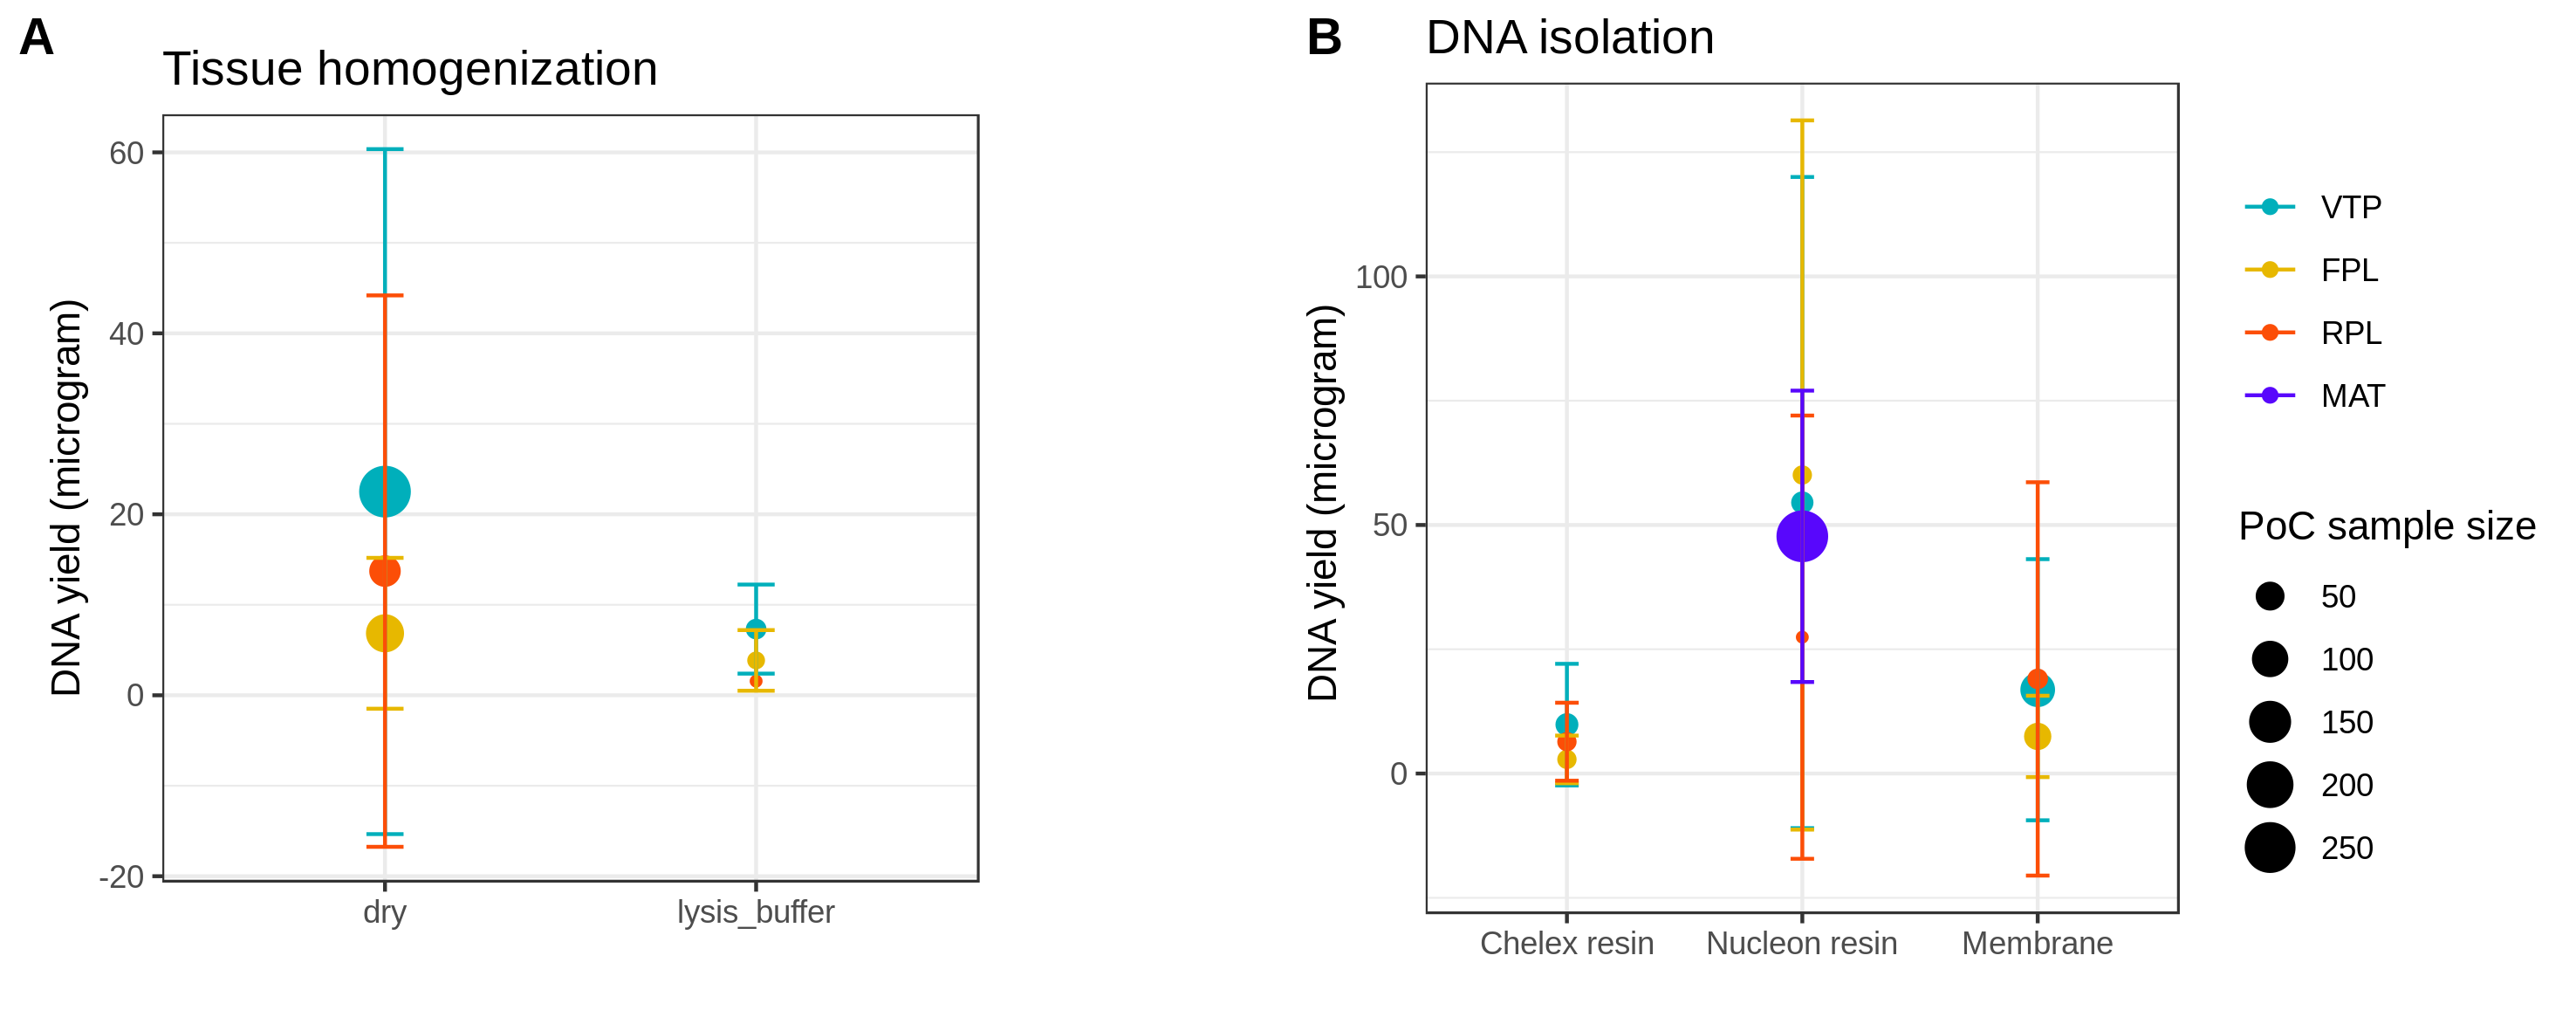
\includegraphics[width= 14 cm, high= 16cm]{fig/panelDNA.png}
    \caption{\textbf{Optimization of tissue homogenization and DNA extraction.} We do not observe significant difference between two methods of tissue homogenization (\textbf{A}), and three methods of DNA isolation (\textbf{b}) apart form a slightly higher range of yield for one type of resin. VTP: voluntary pregnancy termination;  FPL: first pregnancy loss; RPL:recurrent pregnancy loss;  MAT: maternal bllod; PoC: product of conception.}
    \label{fig:dna}
\end{figure}


%\begin{figure}[ht]
%    \centering
%    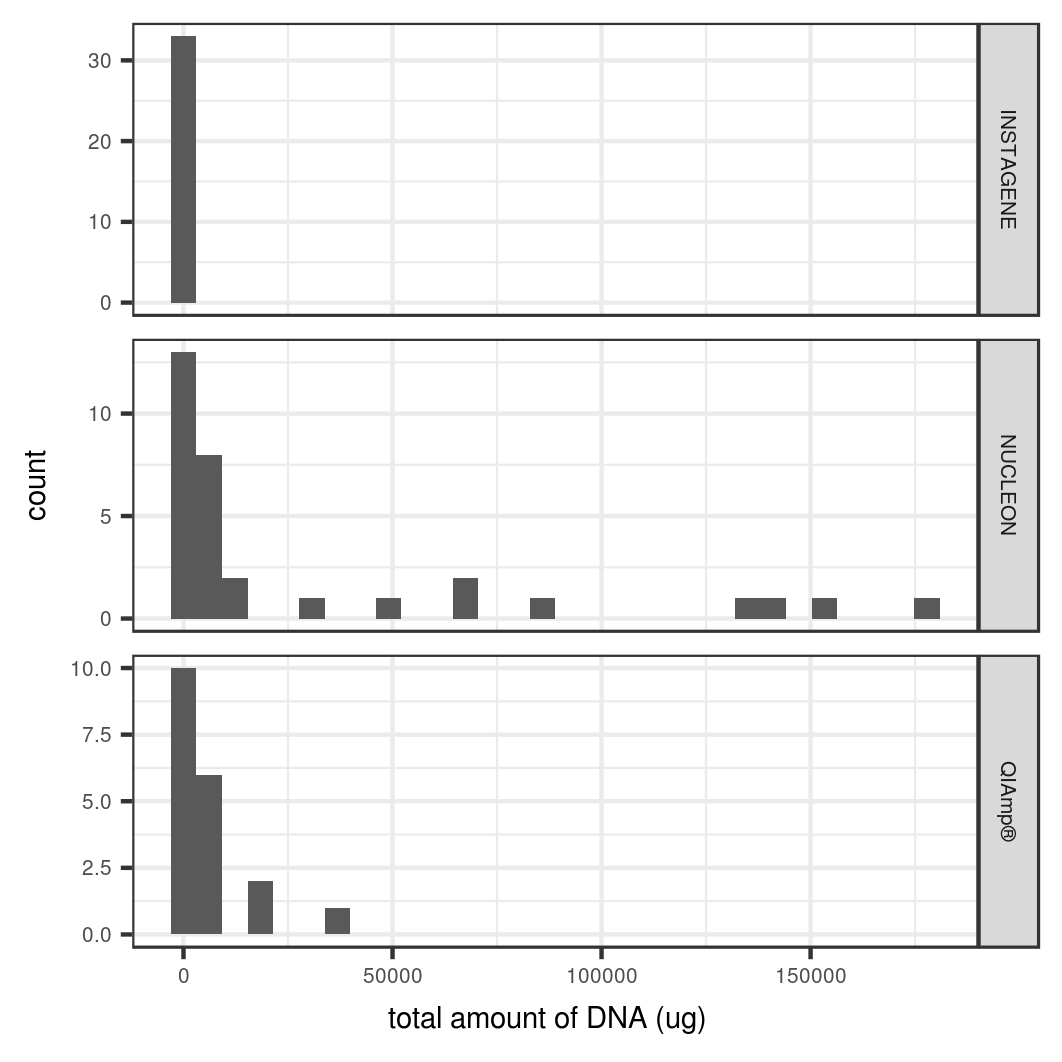
\includegraphics[width= 14 cm, high= 16cm]{fig/totaldna_bykit.png}
%    \caption{\textbf{Yeld of DNA extraction form chorionic villi by extraction kit.} Distributions of total DNA as quantified using the  Qubit 2.0 Fluorometer} 
%    \label{fig:dnayeld}
%\end{figure}


\begin{figure}[ht]
    \centering
    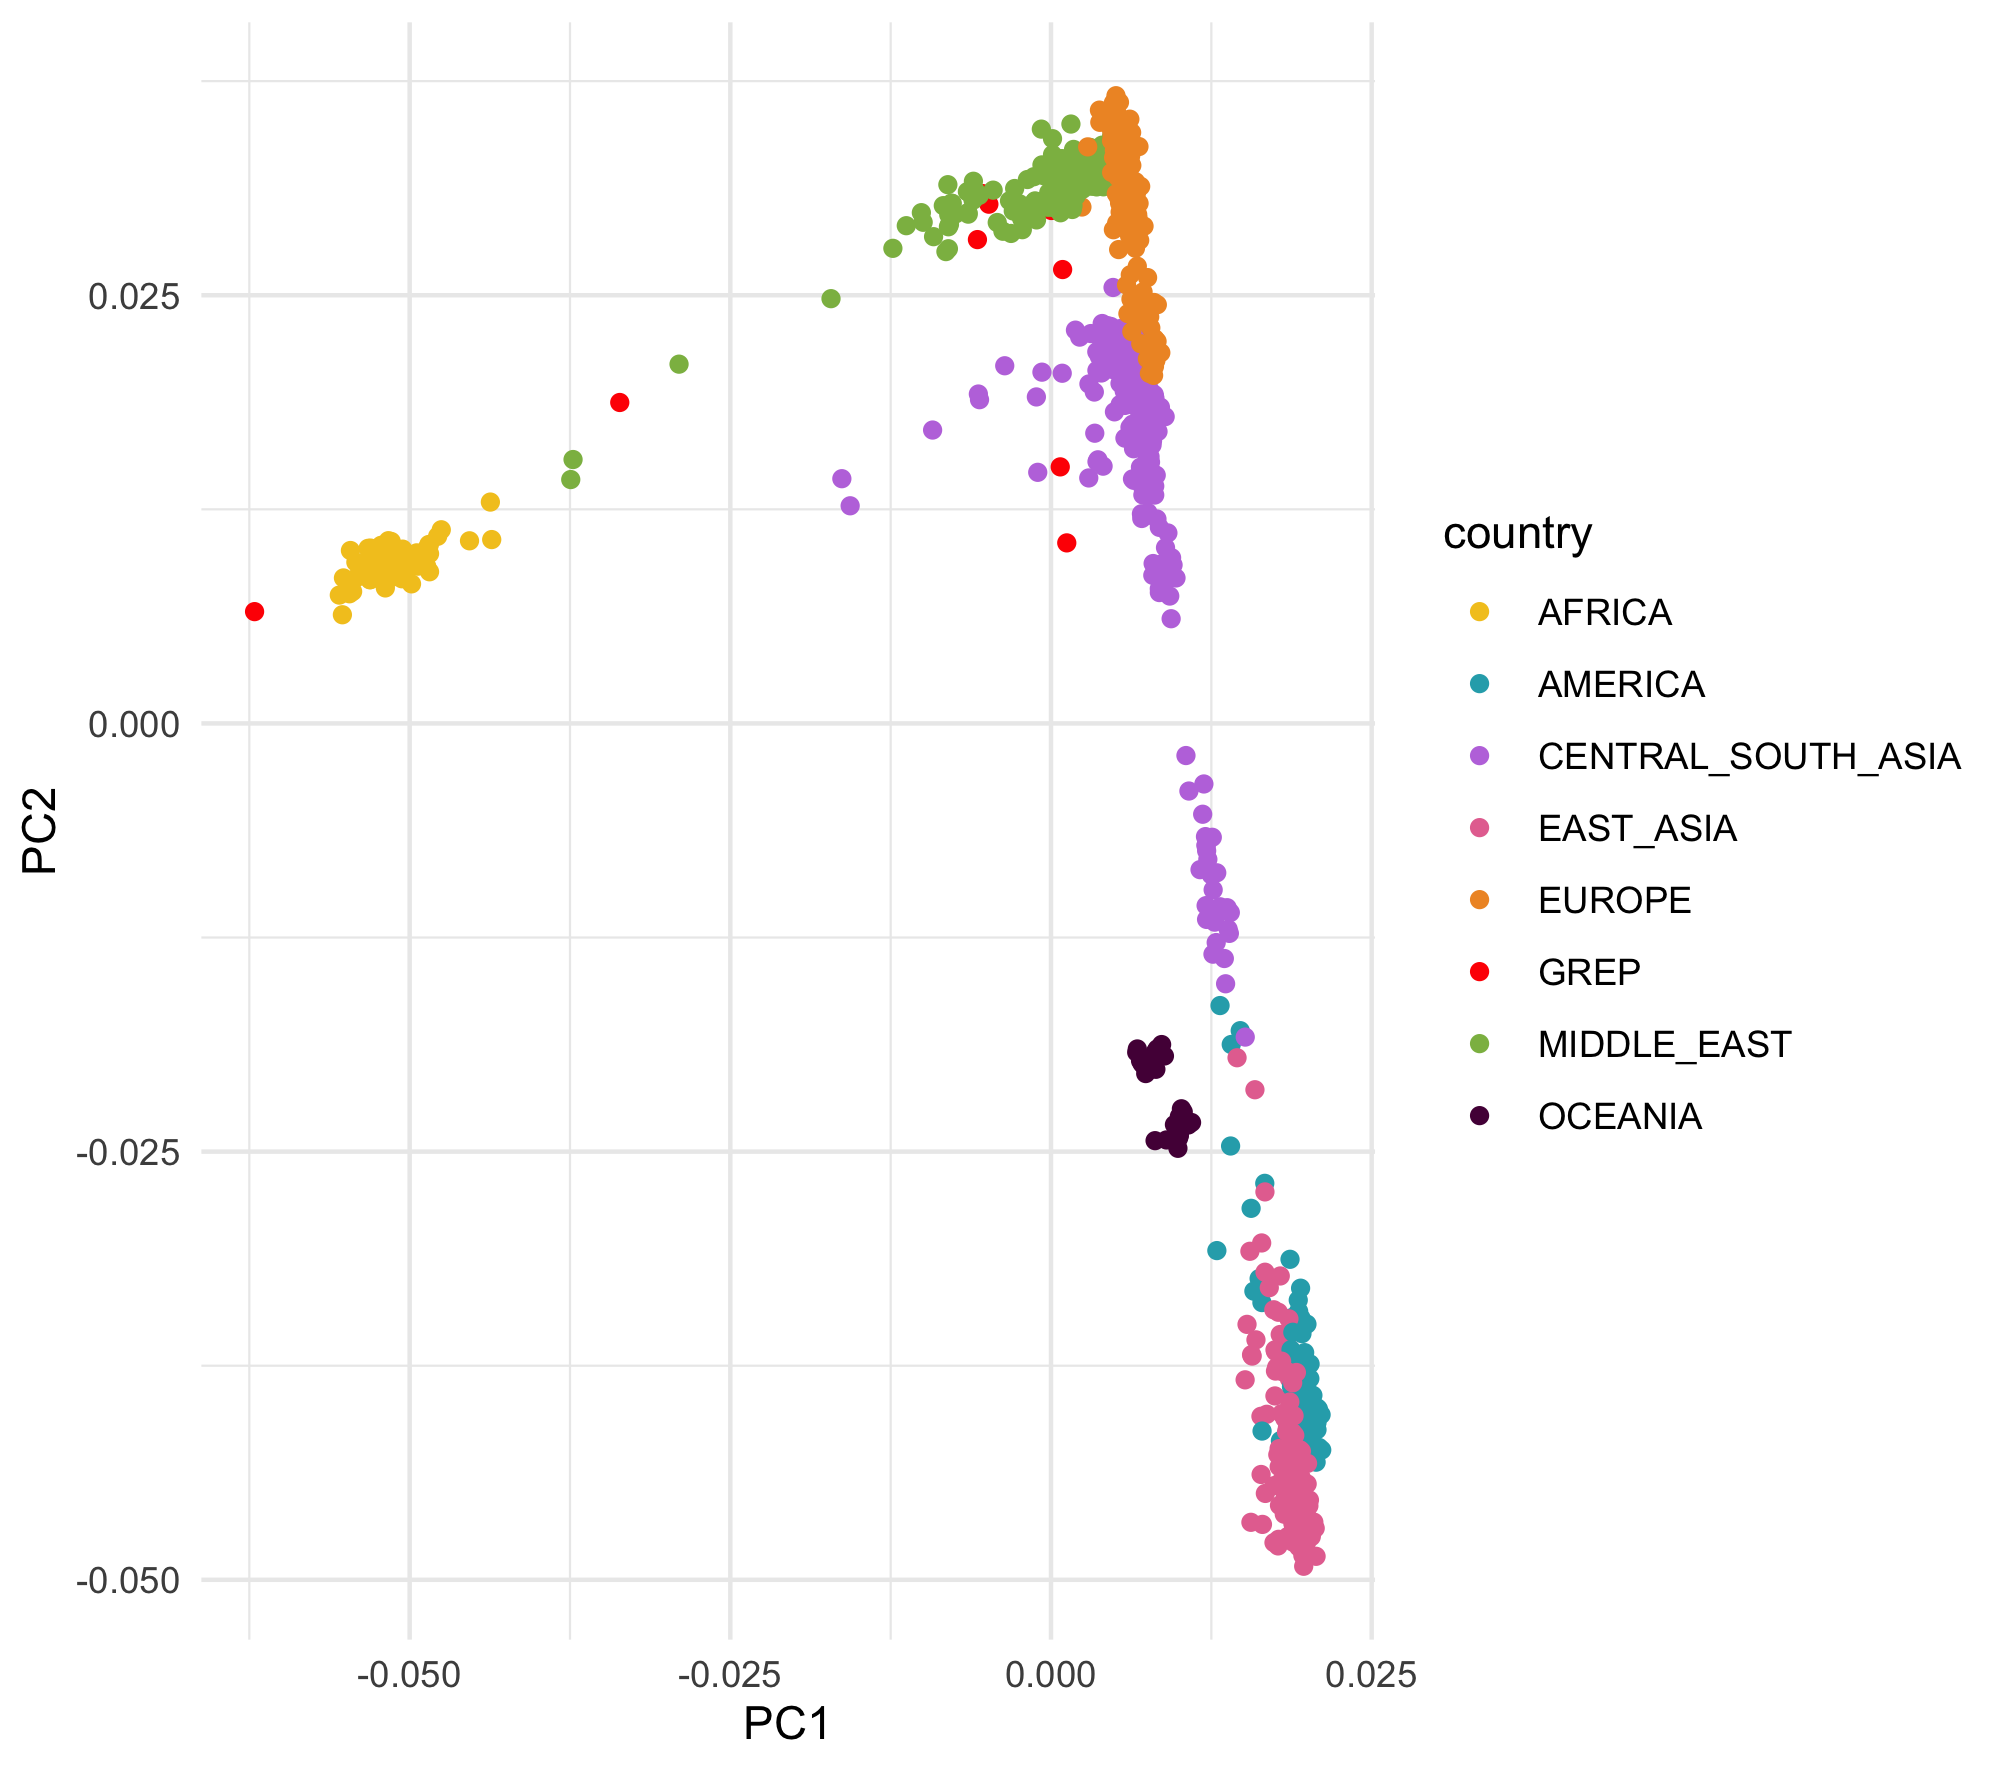
\includegraphics[width= 14 cm, high= 16cm]{fig/pca_hgdp-grep_noALPHA.png}
    \caption{\textbf{Principal Component Analysis.} Plot of the first and second components obtained using 1,2M autosomal SNPs and considering genomic data of the ten embryos sequenced in this study and publicly available data of individuals form the Human Genome Diversity Project}
    \label{fig:pca}
\end{figure}


\begin{figure}[ht]
    \centering
    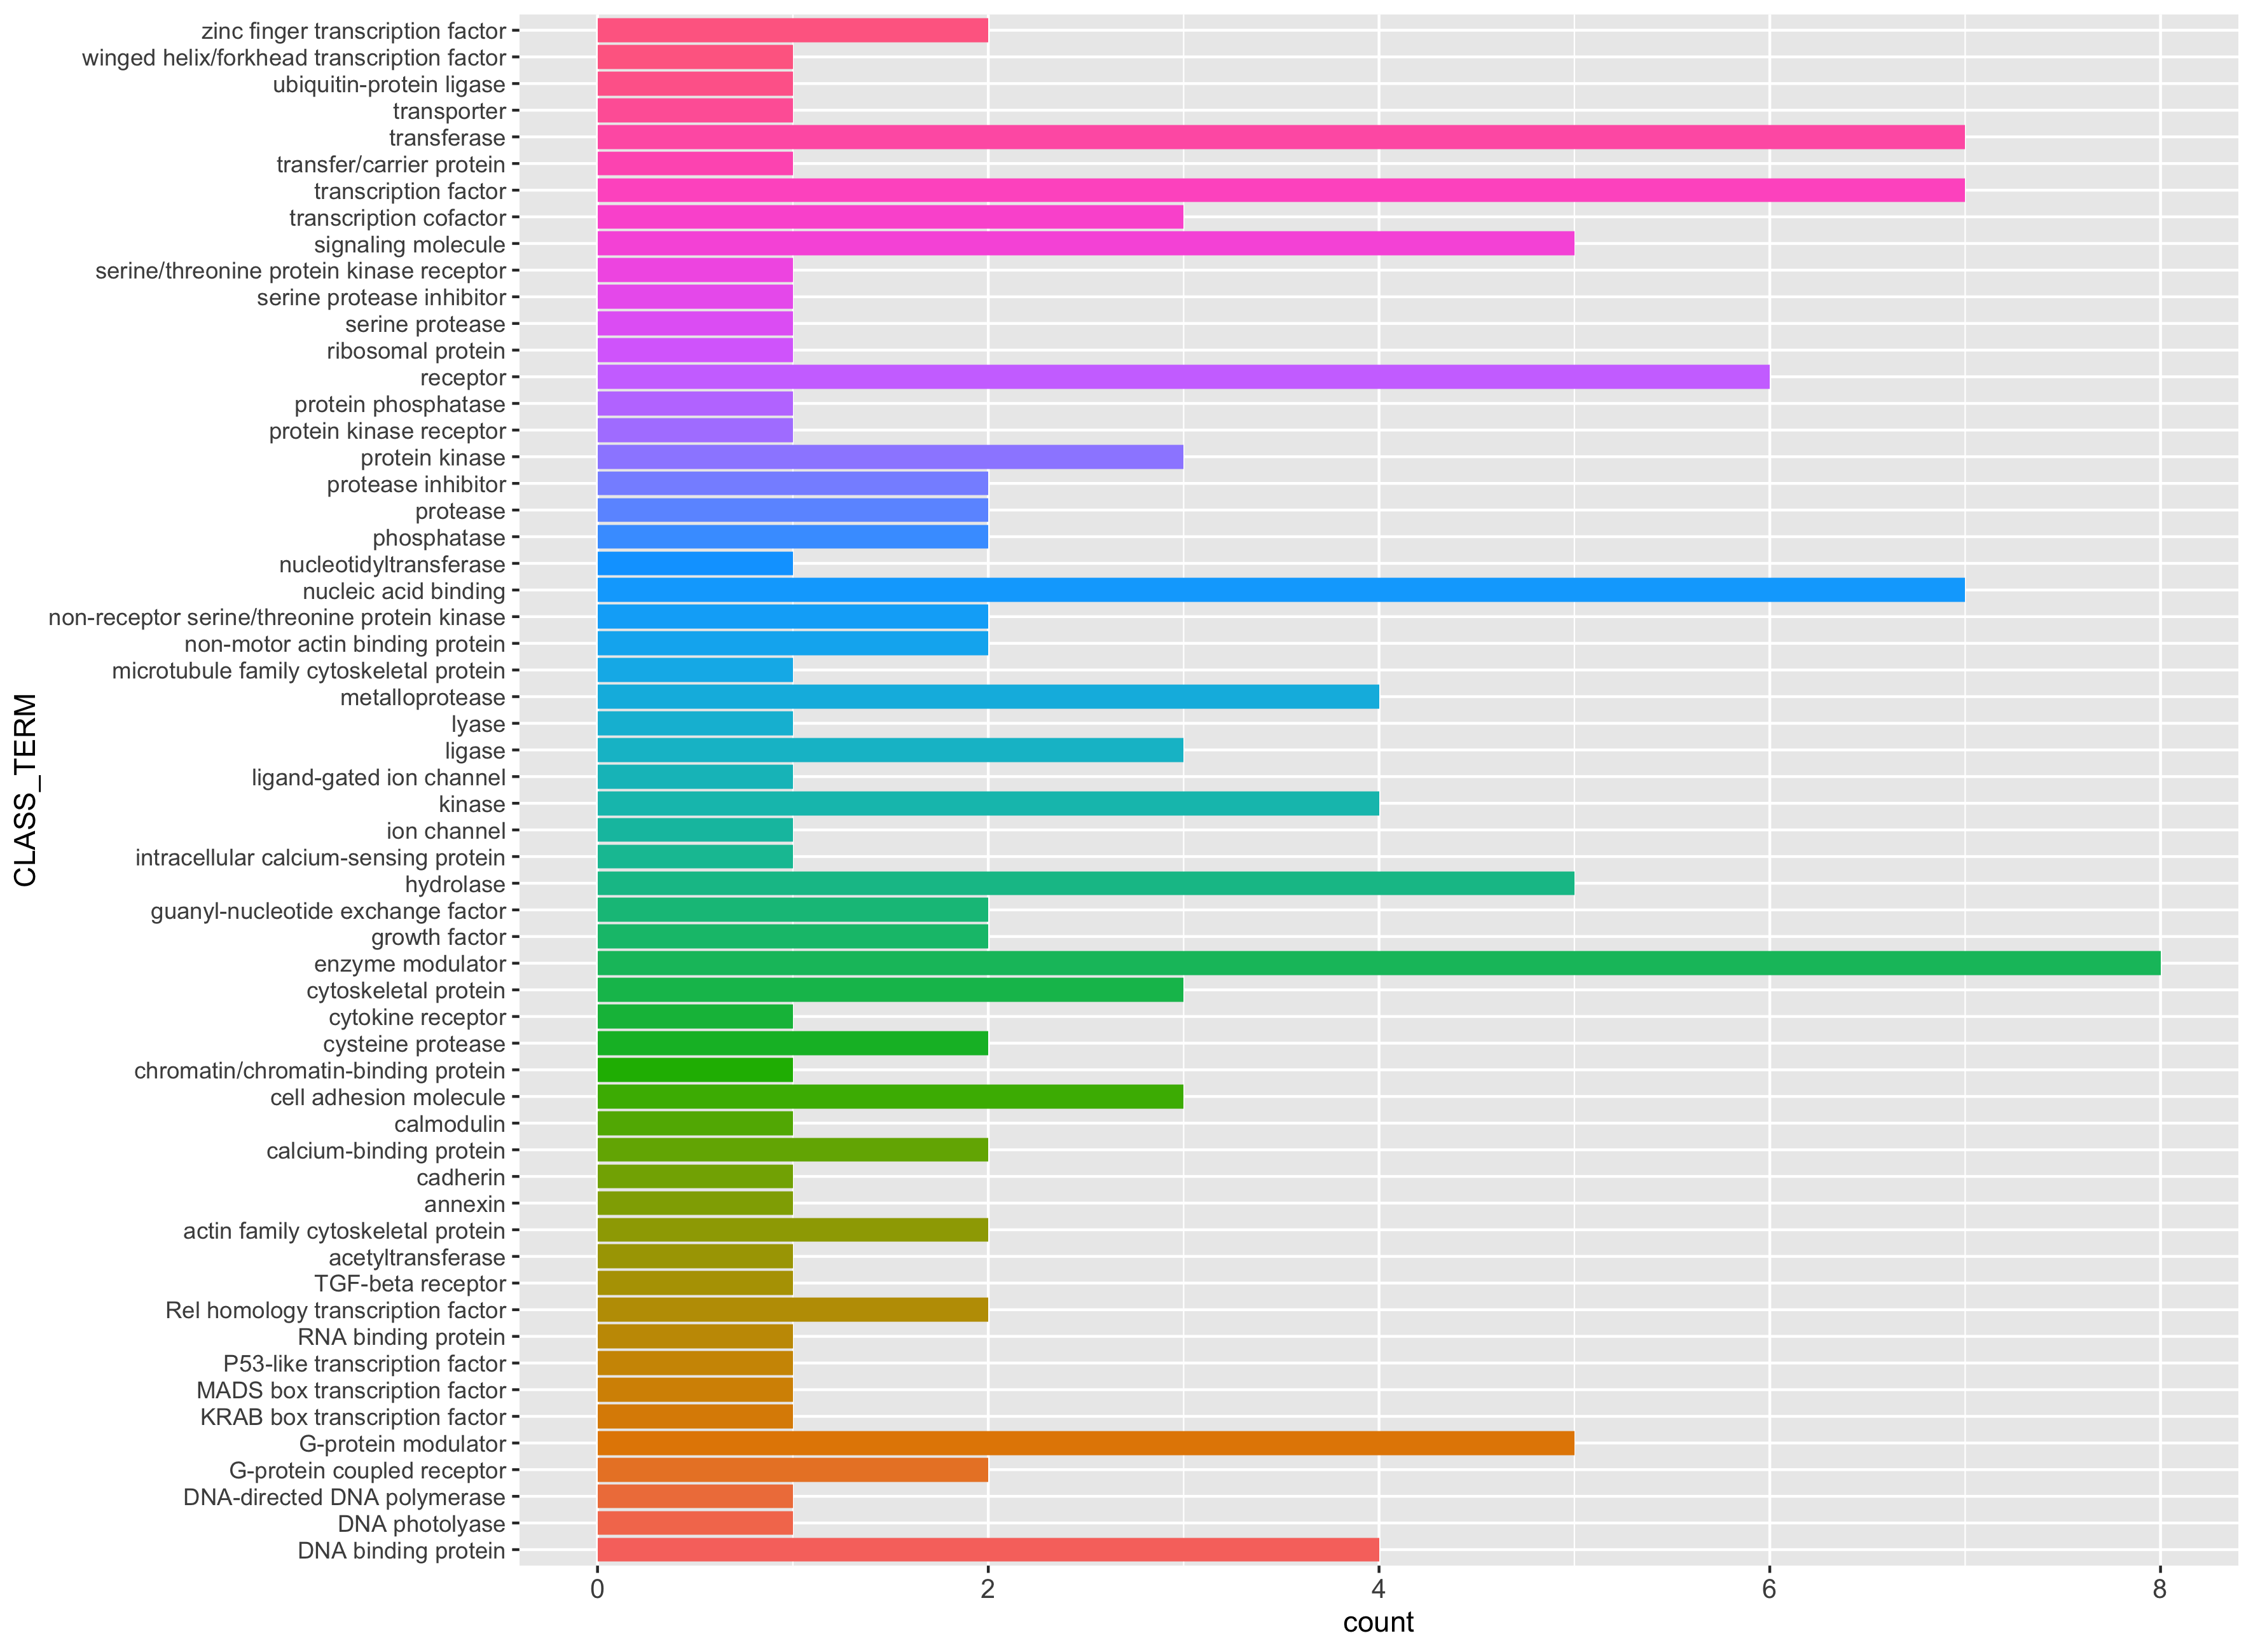
\includegraphics[width= 14 cm, high= 16cm]{fig/class_term_grep.png}
    \caption{\textbf{Classification of the prioritized genes by protein class. }}
    \label{fig:protClass}
\end{figure}




%\begin{figure}[ht]
%    \centering
%    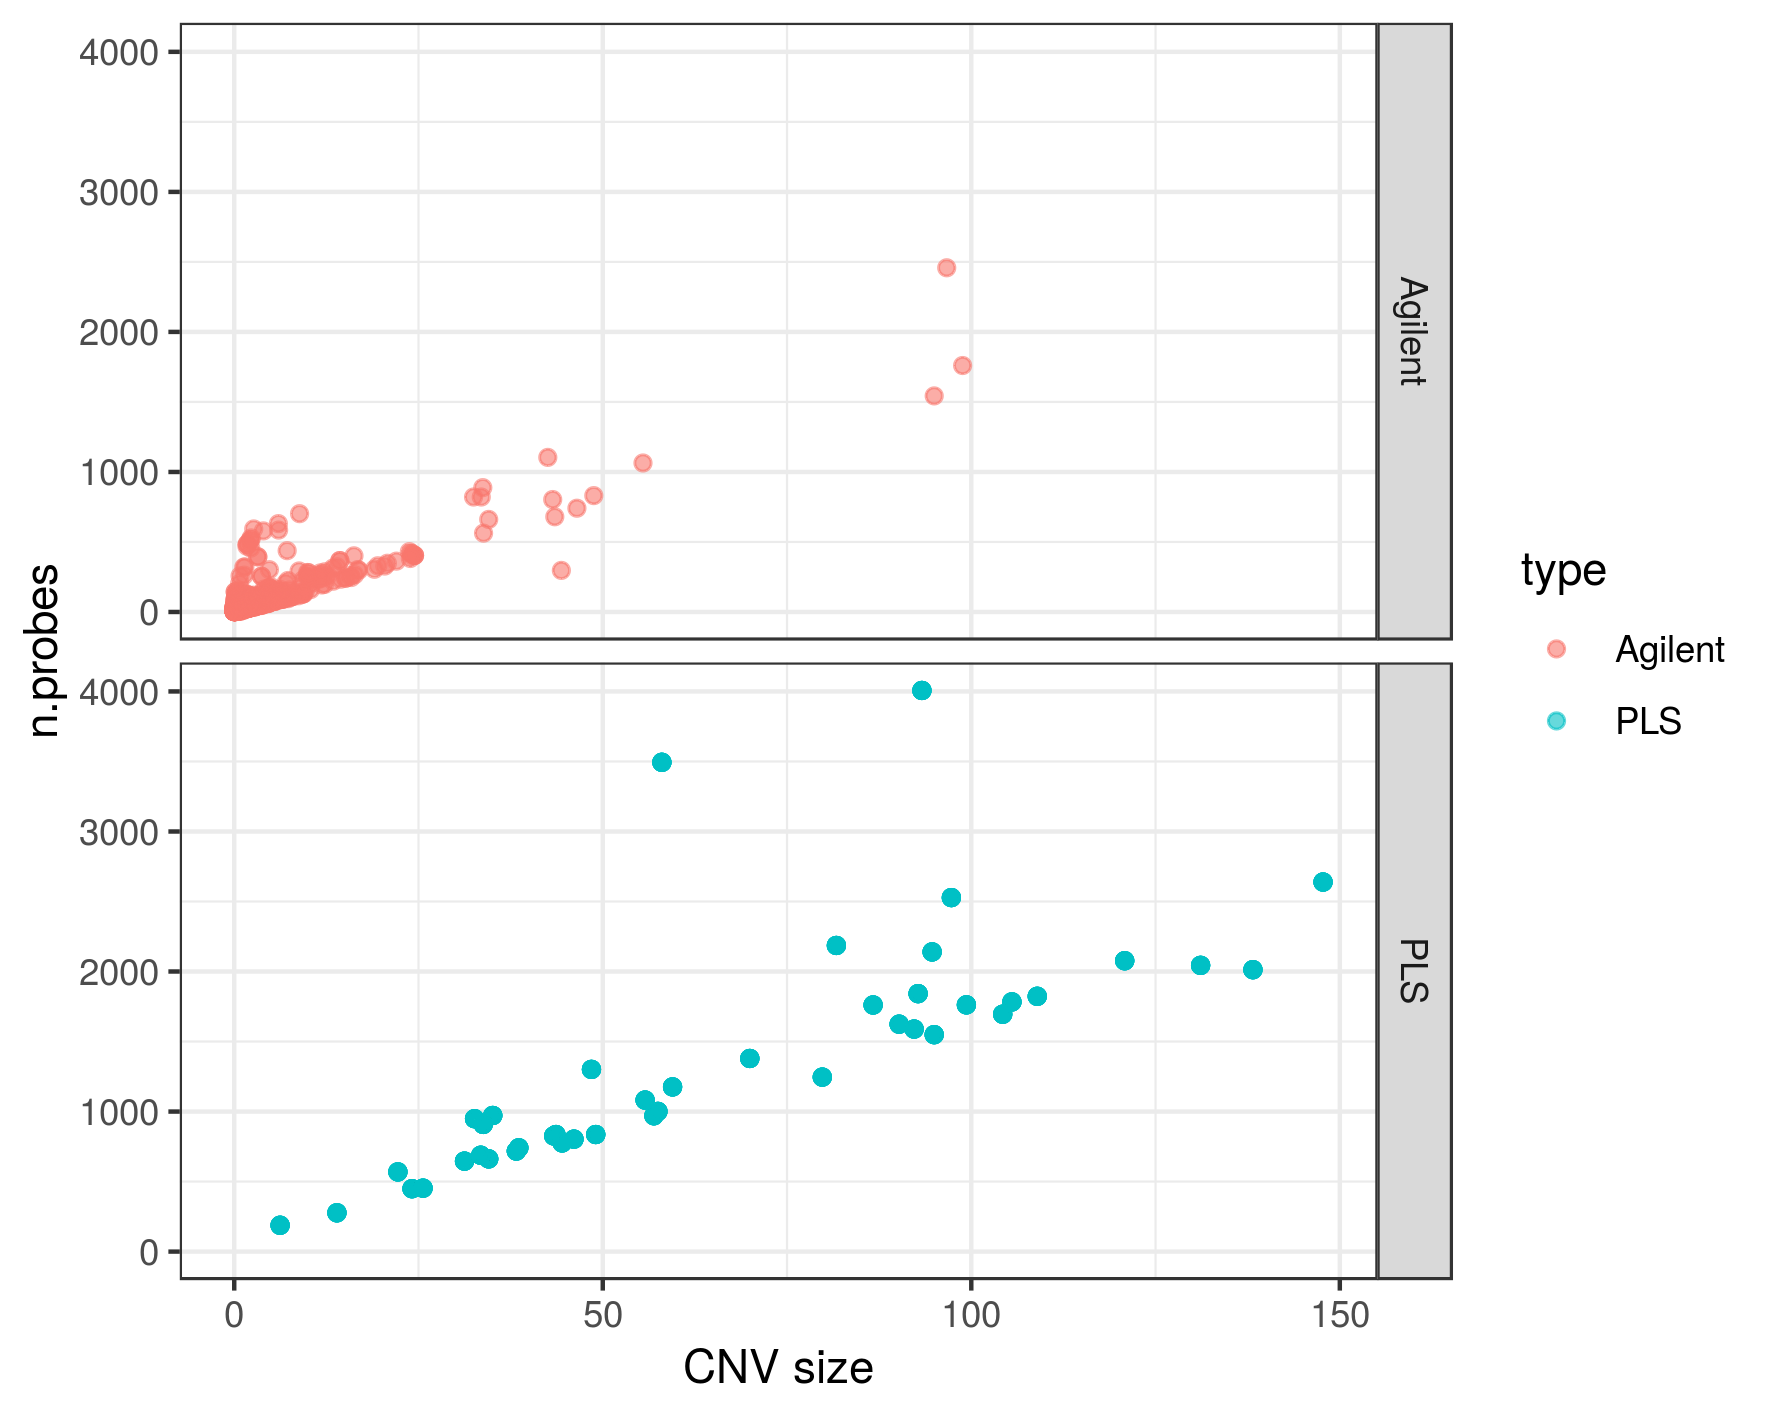
\includegraphics[width= 14 cm, high= 16cm]{fig/cnvCallComparison.png}
%    \caption{\textbf{Copy number variant detection.} Comparison of calls made by the Agilent software and the penalized least square method implemented in the copynumber R package \cite{nilsen2012copynumber}} 
%    \label{fig:cnvmethods}
%\end{figure}